\documentclass{article}

\usepackage{fancyhdr}
\usepackage{extramarks}
\usepackage{amsmath}
\usepackage{amsthm}
\usepackage{amsfonts}
\usepackage{tikz}
\usepackage[plain]{algorithm}
\usepackage{algpseudocode}
\usepackage{graphicx}
\usetikzlibrary{automata,positioning}
\usepackage{pdfpages}

%
% Basic Document Settings
%

\topmargin=-0.45in
\evensidemargin=0in
\oddsidemargin=0in
\textwidth=6.5in
\textheight=9.0in
\headsep=0.25in

\linespread{1.1}

\pagestyle{fancy}
\lhead{\hmwkAuthorName}
\chead{\hmwkClass\ (\hmwkClassInstructor\ \hmwkClassTime): \hmwkTitle}
\rhead{\firstxmark}
\lfoot{\lastxmark}
\cfoot{\thepage}

\renewcommand\headrulewidth{0.4pt}
\renewcommand\footrulewidth{0.4pt}

\setlength\parindent{0pt}

%
% Create Problem Sections
%

\newcommand{\enterProblemHeader}[1]{
    \nobreak\extramarks{}{Problem \arabic{#1} continued on next page\ldots}\nobreak{}
    \nobreak\extramarks{Problem \arabic{#1} (continued)}{Problem \arabic{#1} continued on next page\ldots}\nobreak{}
}

\newcommand{\exitProblemHeader}[1]{
    \nobreak\extramarks{Problem \arabic{#1} (continued)}{Problem \arabic{#1} continued on next page\ldots}\nobreak{}
    \stepcounter{#1}
    \nobreak\extramarks{Problem \arabic{#1}}{}\nobreak{}
}

\setcounter{secnumdepth}{0}
\newcounter{partCounter}
\newcounter{homeworkProblemCounter}
\setcounter{homeworkProblemCounter}{1}
\nobreak\extramarks{Problem \arabic{homeworkProblemCounter}}{}\nobreak{}

%
% Homework Problem Environment
%
% This environment takes an optional argument. When given, it will adjust the
% problem counter. This is useful for when the problems given for your
% assignment aren't sequential. See the last 3 problems of this template for an
% example.
%
\newenvironment{homeworkProblem}[1][-1]{
    \ifnum#1>0
        \setcounter{homeworkProblemCounter}{#1}
    \fi
    \section{Problem \arabic{homeworkProblemCounter}}
    \setcounter{partCounter}{1}
    \enterProblemHeader{homeworkProblemCounter}
}{
    \exitProblemHeader{homeworkProblemCounter}
}

%
% Homework Details
%   - Title
%   - Due date
%   - Class
%   - Section/Time
%   - Instructor
%   - Author
%

\newcommand{\hmwkTitle}{Homework\ \#3}
\newcommand{\hmwkDueDate}{September 29, 2019}
\newcommand{\hmwkClass}{CMSE 820}
\newcommand{\hmwkClassTime}{}
\newcommand{\hmwkClassInstructor}{Professor Yuying Xie}
\newcommand{\hmwkAuthorName}{\textbf{Boyao Zhu}}

%
% Title Page
%

\title{
    \vspace{2in}
    \textmd{\textbf{\hmwkClass:\ \hmwkTitle}}\\
    \normalsize\vspace{0.1in}\small{Due\ on\ \hmwkDueDate\ at 11:59pm}\\
    \vspace{0.1in}\large{\textit{\hmwkClassInstructor\ \hmwkClassTime}}
    \vspace{3in}
}

\author{\hmwkAuthorName}
\date{}

\renewcommand{\part}[1]{\textbf{\large Part \Alph{partCounter}}\stepcounter{partCounter}\\}

%
% Various Helper Commands
%

% Useful for algorithms
\newcommand{\alg}[1]{\textsc{\bfseries \footnotesize #1}}

% For derivatives
\newcommand{\deriv}[1]{\frac{\mathrm{d}}{\mathrm{d}x} (#1)}

% For partial derivatives
\newcommand{\pderiv}[2]{\frac{\partial}{\partial #1} (#2)}

% Integral dx
\newcommand{\dx}{\mathrm{d}x}

% Alias for the Solution section header
\newcommand{\solution}{\textbf{\large Solution}}

% Probability commands: Expectation, Variance, Covariance, Bias
\newcommand{\E}{\mathrm{E}}
\newcommand{\Var}{\mathrm{Var}}
\newcommand{\Cov}{\mathrm{Cov}} 
\newcommand{\Bias}{\mathrm{Bias}}

\begin{document}

\maketitle

\pagebreak

\begin{homeworkProblem}

1. \textbf{Solution}\\
Start from the truncated power series:
\[
f(X) = \sum_{j=0}^{3}\beta_jX^j+\sum_{k=1}^{K}\theta_k(X-\xi_k)_+^3
\]
For the left boundary knot
\[
f(X) = \sum_{j=0}^{3}\beta_jX^j,\qquad X\leq\xi_i
\]
and we need the constraints \(\beta_2=0\) and \(\beta_3=0\) for the function to be linear.
\\
For the right boundary knot
\[
\begin{split}
f(X) &= \sum_{j=0}^{3}\beta_jX^j+\sum_{k=1}^{K}\theta_k(X-\xi_k)_+^3, \qquad X\geq\xi_i\\
       &= \sum_{j=0}^{3}\beta_jX^j+\sum_{k=1}^{K}\theta_kX^3-\sum_{k=1}^K\theta_k\xi_k3X^2+\sum_{k=1}^K\theta_k\xi_k^23X-\sum_{k=1}^K\theta_k\xi_k^3
\end{split}
\]
and we need the constraints \(\theta_k=0\ \text{and} \sum_{k=1}^K\xi_k\theta_k=0\) for the function to be linear.\\
Hence, the truncated power series representation
\[
f(X) = \sum_{j=0}^{3}\beta_jX^j+\sum_{k=1}^{K}\theta_k(X-\xi_k)_+^3
\]
with the constraints on the coefficients
\[
\beta_2=0,\qquad \beta_3=0, \qquad \sum_{k=1}^K\theta_k=0, \qquad \sum_{k=1}^K\xi_k\theta_k=0
\]
\\
2.  \textbf{Solution}\\
Taking into account first the \(\beta\) restrictions, we can construct a new basis with the first two basis function as 
\[
f(X) = \beta_0\cdot\underbrace{1}_{N_1(x)}+\beta_1\cdot\underbrace{X}_{N_2(x)}+0\cdot X^2+0\cdot X^3 + \cdots
\]
For the \(\theta\) constraints, we utilize that
\[
\sum_{k=1}^{K-2}\theta_k = -\theta_{K-1}-\theta_{K}, \qquad \sum_{k=1}^{K-2}\xi_k\theta_k=-\xi_{K-1}\theta_{K-1}-\xi_K\theta_K
\]
Take out the last two terms of the truncated basis functions:\\
For the \(\theta\) constraints, we utilize that
\[
\sum_{k=1}^K\theta_k(X-\xi_k)^3_+ = \sum_{k=1}^{K-2}\theta_k(X-\xi_k)^3_++\theta_{K-1}(X-\xi_{K-1})^3_++\theta_K(X-\xi_K)^3_+
\]
Start with the second last term 
\[
\begin{split}
\theta_{K-1}(X-\xi_{K-1})^3_+ &= \frac{(X-\xi_{K-1})^3_+}{(\xi_K-\xi_{K-1})}\big(\theta_{K-1}(\xi_K-\xi_{K-1})\big)\\
&=  \frac{(X-\xi_{K-1})^3_+}{(\xi_K-\xi_{K-1})}\Big(\theta_{K-1}\xi_K-\theta_{K-1}\xi_{K-1}+\underbrace{\theta_K\xi_K-\theta_K\xi_K}_0\Big)\\
&= \frac{(X-\xi_{K-1})^3_+}{(\xi_K-\xi_{K-1})}\big(\xi_K(\theta_{K-1}+\theta_K)-\xi_{K-1}\theta_{K-1}-\xi_K\theta_K\big)\\
&= \frac{(X-\xi_{K-1})^3_+}{(\xi_K-\xi_{K-1})} \Big(-\xi_K\sum_{k=1}^{K-2}\theta_k+\sum_{k=1}^{K-2}\theta_k\xi_k\Big)  \qquad \text{by constraints}\\
&= -\frac{(X-\xi_{K-1})^3_+}{(\xi_K-\xi_{K-1})}\sum_{k=1}^{K-2}\theta_k(\xi_K-\xi_k)\\
&= -\sum_{k=1}^{K-2}\theta_k(\xi_K-\xi_k)\frac{(X-\xi_{K-1})^3_+}{(\xi_K-\xi_{K-1})}
\end{split}
\]
Then, take the last term, and do the same
\[
\begin{split}
\theta_K(X-\xi_K)^3_+ &= \frac{(X-\xi_{K})^3_+}{(\xi_K-\xi_{K-1})}\Big(\theta_K\xi_K-\theta_K\xi_{K-1}+\underbrace{\theta_{K-1}\xi_{K-1}-\theta_{K-1}\xi_{K-1}}_0\Big)\\
&= \frac{(X-\xi_{K})^3_+}{(\xi_K-\xi_{K-1})}\big(-\xi_{K-1}(\theta_{K-1}+\theta_K)+\xi_{K-1}\theta_{K-1}+\xi_{K}\theta_K\big)\\
&= \frac{(X-\xi_{K})^3_+}{(\xi_K-\xi_{K-1})}\Big(\xi_{K-1}\sum_{k=1}^{K-2}\theta_k-\sum_{k=1}^{K-2}\theta_k\xi_k\Big)  \qquad \text{by constraints}\\
&= (X-\xi_{K})^3_+\sum_{k=1}^{K-2}\theta_k\frac{\xi_{K-1}-\xi_k}{(\xi_K-\xi_{K-1})}\\
&= (X-\xi_{K})^3_+\sum_{k=1}^{K-2}\theta_k(\xi_K-\xi_k)\frac{\xi_{K-1}-\xi_k+\xi_K-\xi_K}{(\xi_K-\xi_{K-1})(\xi_K-\xi_k)}\\
&= (X-\xi_{K})^3_+\sum_{k=1}^{K-2}\theta_k(\xi_K-\xi_k)\Big(\frac{1}{\xi_K-\xi_{K-1}}-\frac{1}{\xi_K-\xi_k}\Big)
\end{split}
\]
Then, we combine the two expressions
\[
\begin{split}
\sum_{k=1}^K\theta_k(X-\xi_k)^3_+ &= \sum_{k=1}^{K-2}\theta_k(X-\xi_k)^3_++\theta_{K-1}(X-\xi_{K-1})^3_++\theta_K(X-\xi_K)^3_+\\
&=  \sum_{k=1}^{K-2}\theta_k(X-\xi_k)^3_+ -\sum_{k=1}^{K-2}\theta_k(\xi_K-\xi_k)\frac{(X-\xi_{K-1})^3_+}{(\xi_K-\xi_{K-1})}\\
&+(X-\xi_{K})^3_+\sum_{k=1}^{K-2}\theta_k(\xi_K-\xi_k)\Big(\frac{1}{\xi_K-\xi_{K-1}}-\frac{1}{\xi_K-\xi_k}\Big)\\
&=  \sum_{k=1}^{K-2}\theta_k(\xi_K-\xi_k)\frac{(X-\xi_k)^3_+}{\xi_K-\xi_k} -\sum_{k=1}^{K-2}\theta_k(\xi_K-\xi_k)\frac{(X-\xi_{K-1})^3_+}{(\xi_K-\xi_{K-1})}\\
&+  \sum_{k=1}^{K-2}\theta_k(\xi_K-\xi_k)\Big(\frac{(X-\xi_{K})^3_+}{\xi_K-\xi_{K-1}}-\frac{(X-\xi_{K})^3_+}{\xi_K-\xi_k}\Big)\\
&=  \sum_{k=1}^{K-2}\theta_k(\xi_K-\xi_k)\Big(\frac{(X-\xi_k)^3_+}{\xi_K-\xi_k}-\frac{(X-\xi_{K-1})^3_+}{(\xi_K-\xi_{K-1})}+\frac{(X-\xi_{K})^3_+}{\xi_K-\xi_{K-1}}-\frac{(X-\xi_{K})^3_+}{\xi_K-\xi_k}\Big)\\
&=  \sum_{k=1}^{K-2}\theta_k(\xi_K-\xi_k)\Big(\frac{(X-\xi_k)^3_+-(X-\xi_K)^3_+}{\xi_K-\xi_k}-\frac{(X-\xi_{K-1})^3_+-(X-\xi_{K})^3_+}{\xi_K-\xi_{K-1}}
\end{split}
\]
Therefore,
\[
\sum_{k=1}^K\theta_k(X-\xi_k)^3_+ = \sum_{k=1}^{K-2}\theta_k(\xi_K-\xi_k)(d_k(X)-d_{K-1}(X))
\]
where
\[
N_{k+2}(X) = d_k(X)-d_{K-1}(X), \qquad
d_k(X)=\frac{(X-\xi_k)^3_+-(X-\xi_K)_+^3}{\xi_K-\xi_k}
\]
\\
3.  \textbf{Solution}\\
It is easy to verify that the second derivative of basis functions exist and equal 0 at both \(\xi_1 \text{and } \xi_K\).  Thus these basis functions satisfy the requirement of Natural Cubic spline.

\end{homeworkProblem}



\begin{homeworkProblem}
2.  \textbf{Solution}\\
At first, \(x_0=a\), \(x_{N+1}=b\), and \(f_i=f^{'''}(x)\).  And for \(x\in[x_i, x_{i+1}]\).  Also we have \(h(x_i)=\tilde{f}(x_i)-f(x_i) = y_i-y_i = 0\)
\[
\begin{split}
\int_a^bf^{''}(x)h^{''}(x)dx &= f^{''}(x)h^{'}(x)\rvert_a^b - \int_a^b f^{'''}(x)h^{'}(x)dx\\
&= \sum_{i=0}^N\int_{x_i}^{x_{i+1}}f^{'''}(x)h^{'}(x)dx   \qquad (f^{''}(a)=f^{''}(b)=0)\\
&= \sum_{i=0}^N f_i \int_{x_i}^{x_{i+1}}h^{'}(x)dx   \\
&= \sum_{i=0}^N f_i [h(x_{i+1})-h(x_i)] \\
&= 0
\end{split}
\]

3.  \textbf{Solution}\\
\[
\begin{split}
\int_a^bf^{''}(x)^2 &\leq \int_a^b\tilde{f}^{''}(x)^2dx \\
& \leq \int_a^b (f^{''}(x)+h^{''}(x))^2 dx \\
& \leq \int_a^b f^{''}(x)^2 + h^{''}(x)^2 + 2f^{''}(x)h^{''}(x)dx\\
& \leq \int_a^b f^{''}(x)^2 + h^{''}(x)^2dx  \qquad (by (b))
\end{split}
\]
This is trivial and the equality holds when \(h^{''}(x)=0\) or \(\tilde{f}(X)-f(X)\).

\end{homeworkProblem}

\begin{homeworkProblem}
The code is attached in the back.
Prediction error for OLS \(= 30.037394792483873\)\\
Prediction error for ridge \(=  25.856854295473653\)\\
Prediction error for lasso \(=  148.39318958116104\)\\
Note that in this case, Ridge outperforms OLS.  But Lasso leads to worst performance.

\end{homeworkProblem}

\begin{homeworkProblem}
\textbf{4a}\\
Cubic Spline\\
\[
\begin{split}
h_1(X) &= 1\\
h_2(X) &= X\\
h_3(X) &= X^2\\
h_4(X) &= X^3\\
h_5(X) &= (X-\frac{\pi}{4})^3_+\\
h_6(X) &= (X-\frac{\pi}{2})^3_+\\
h_7(X) &= (X-\pi)^3_+\\
h_8(X) &= (X-\frac{4\pi}{2})^3_+\\
h_9(X) &= (X-\frac{7\pi}{4})^3_+
\end{split}
\]
Natural Cubic Spline \\
\[
\begin{split}
h_1(X) &= 1\\
h_2(X) &= X\\
h_3(X) &= -\frac{1}{6}(X-\frac{\pi}{4})_+^3+(X-\frac{3\pi}{2})_+^3-\frac{5}{6}(X-\frac{7\pi}{4})_+^3\\
h_4(X) &= -\frac{1}{5}(X-\frac{\pi}{2})_+^3+(X-\frac{3\pi}{2})_+^3-\frac{4}{5}(X-\frac{7\pi}{4})_+^3\\
h_5(X) &= -\frac{1}{3}(X-\pi)_+^3+(X-\frac{3\pi}{2})_+^3-\frac{2}{3}(X-\frac{7\pi}{4})_+^3\\
\end{split}
\]

\end{homeworkProblem}

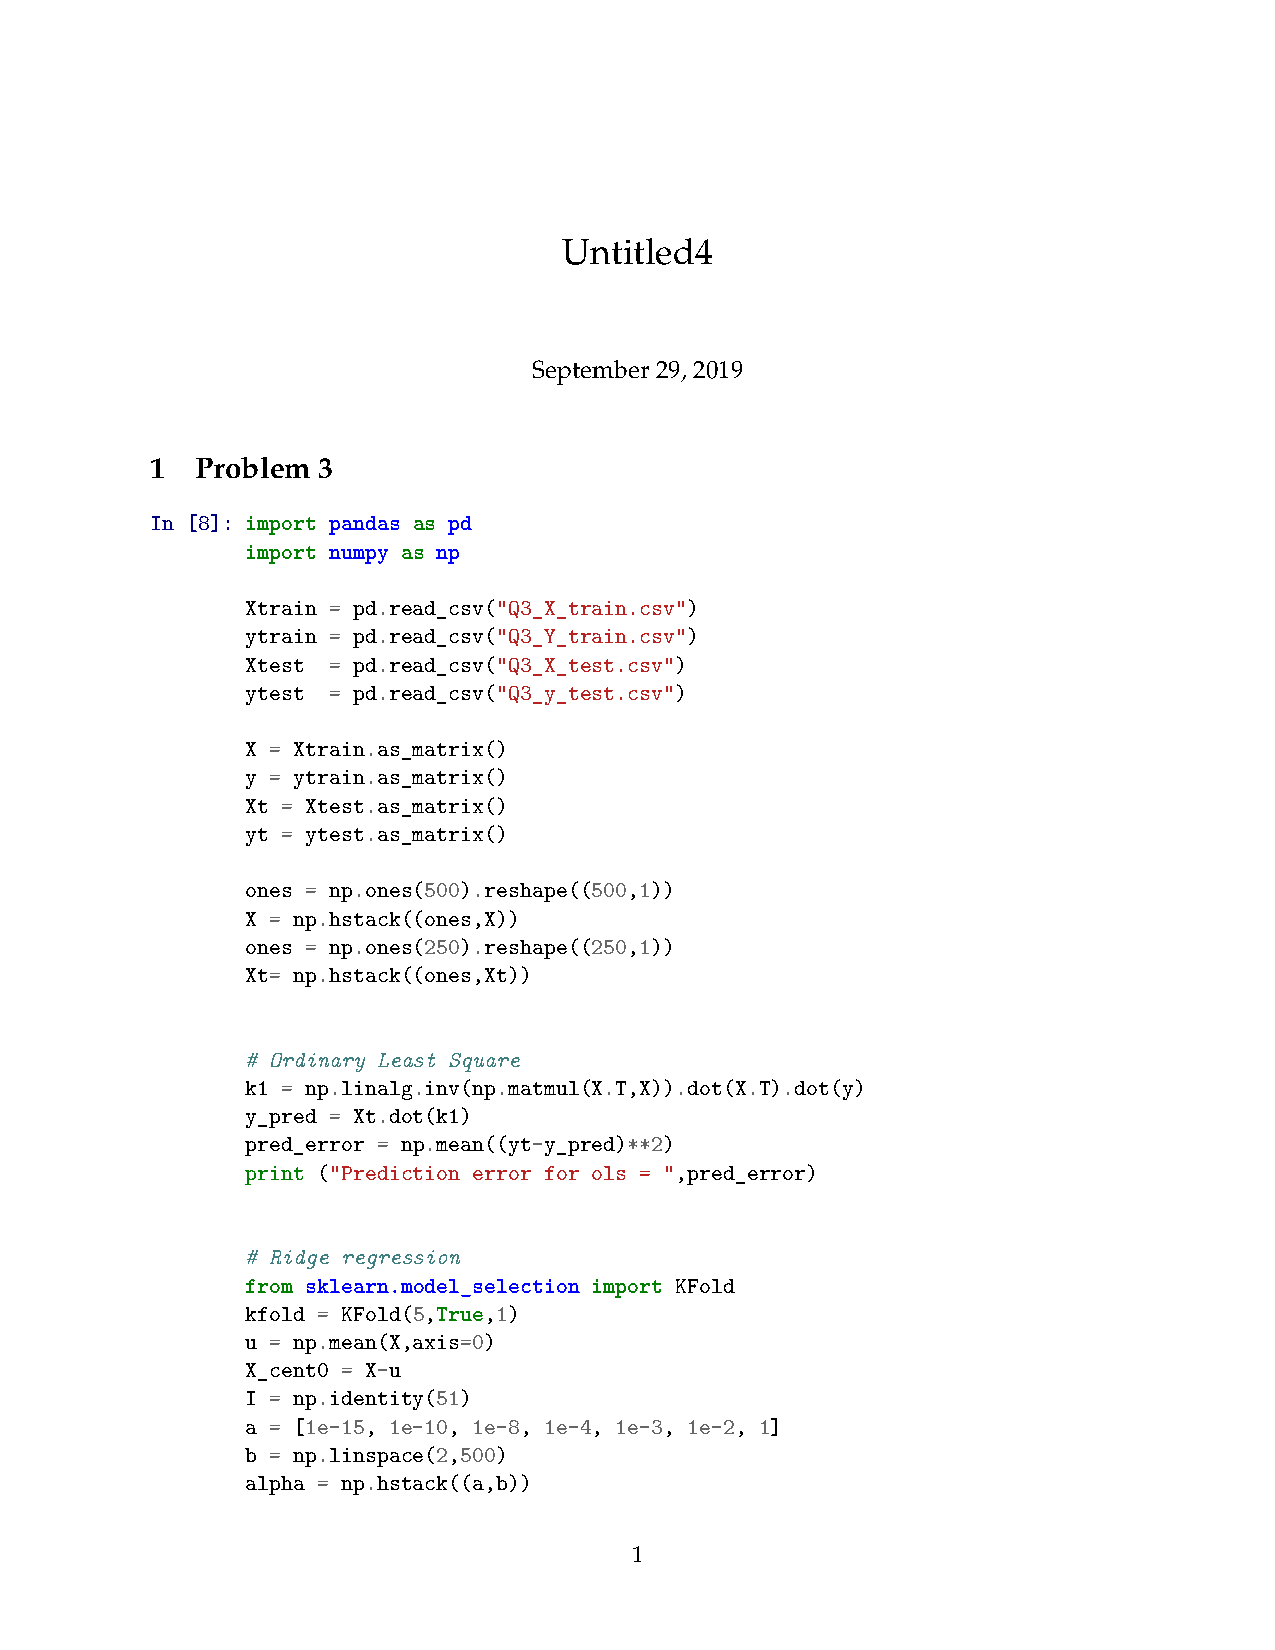
\includepdf[page={-}]{Untitled4.pdf}


\end{document}